% round 4 (panel-r4 NEW-16 / T12): a \clearpage kept the heading off the foot of a page. Round 5 (panel-r5 NEW-7, EIC B1): that
%   \clearpage left a nearly blank page and a page with the heading alone, because two-column floats cannot sit under a heading. It is replaced
%   by a short roadmap, so the heading always has text under it.
% round 7: the roadmap of these tables is the paragraph "Supplementary tables" at the start of sections/app-protocol.tex.
\begin{figure*}[h]
\centering
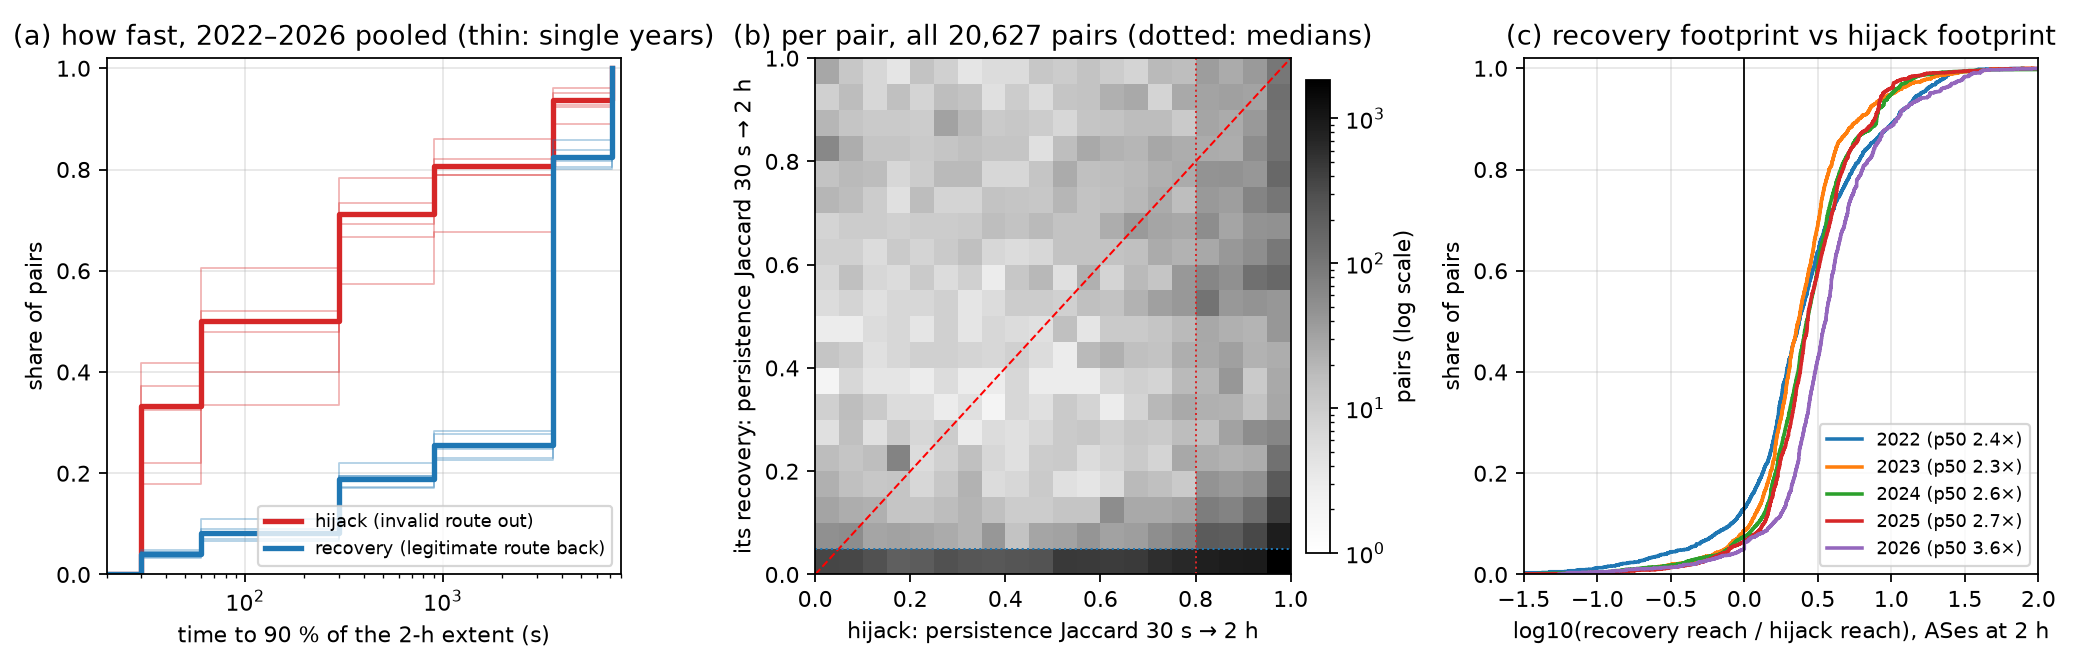
\includegraphics[width=\linewidth]{figures/rpki/recovery_pairs}
\caption{Matched outward and return transitions, 2022--2026. (a) Cumulative distributions of $t_{90}$, pooled over links, with thin lines for single years. (b) Per-link 30-s \floor, outward against return, with a logarithmic density scale, the marginal medians and the diagonal of equal floors. (c) Per-link ratio of return to outward extent by year. Links with undefined timing or ratios are excluded and counted. \Cref{tab:recovery-summary,tab:recovery-gap,tab:recovery-dayblock} give the values by year and by identifier gap.}
\Description{Three panels compare outward and return transitions: timing distributions overlap; per-link early floors scatter on both sides of the diagonal; the return-to-outward extent ratio has medians slightly above one in every year.}
\label{fig:pairs}
\end{figure*}

\begin{table*}[h]
\footnotesize
\centering
\caption{Matched transitions by identifier gap and year. Share of links: of all links of that year. $\Jac_{30}$: 30-s \floor of the outward ($O$) and return ($R$) footprint. Paired $\Delta\Jac$: $R$ minus $O$. Return slower: as in \Cref{tab:recovery-summary}. Intervals: 95\,\% component bootstrap. Row labels: $<1$\,min is below 1\,min, 1--15\,min is at least 1 and below 15\,min, and $\geq 15$\,min is at least 15\,min and below 24\,h.}
\label{tab:recovery-gap}
\setlength{\tabcolsep}{4pt}
\input{generated/recovery_gap_wide.tex}
\end{table*}

\begin{table*}[h]
\footnotesize
\centering
\caption{Recovery intervals with dependence between links (revision analysis). Component: the published bootstrap over connected components of shared events. Day block: UTC days of the outward identifier as resampling units, with days joined by a shared event merged, 10,000 draws. $^{*}$: the pooled extent ratio has no published interval, so this row uses the component bootstrap with 10,000 draws (seed 1701). Gap labels as in \Cref{tab:recovery-gap}: $\geq 15$\,min is at least 15\,min and below 24\,h. Largest units: in 2025, one day holds \num{1013} of the \num{4306} links with a gap under 1\,min. With a gap of at least 15\,min, 116 of \num{1259} links fall on 2024-10-17, with a mean $\Delta\Jac$ of $-0.55$, and 107 of 809 on 2026-08-01, with $-0.18$. Without these days, the means are $+0.09$ and $+0.10$, a post hoc check of these two years only.}
\label{tab:recovery-dayblock}
% round 7 (review-r6 W5, Tables 11-12): the generators (scripts/paper_recovery_dayblock.py, scripts/paper_measurement_checks.py,
%   tools/recovery_gap_wide.py) now print ">= 15 min" for [900, 86400) s; a rerun changed only these labels.
% src: generated/recovery_dayblock.tex header comment (component CI*: 10,000 draws, seed 1701); scripts/paper_recovery_dayblock.py GAPS
%   (gt15min = [900, 86400) s); recovery_dayblock.json years.2025.lt1min (links 4,306, max_links_per_unit 1,013) and years.{2024,2026}.gt15min
%   (links 1,259 / 809, max_links_per_unit 116 / 107). Dates and means: recovery_dayblock.json years.{2024,2026}.gt15min.largest_day
%   (see the src comment in sections/06-recovery.tex): -0.5452 / -0.1827; without the day +0.0924 / +0.0989 (round-3 review NEW-8, X8).
\setlength{\tabcolsep}{4pt}
% Generated by scripts/paper_recovery_dayblock.py; do not edit by hand.
% component CI: the published connected-component bootstrap (1,000 draws, seed 0), reproduced exactly; the
% pooled extent ratio is published without an interval, so its row shows the component bootstrap with
% 10,000 draws, seed 1701 (marked *). day-block CI: UTC days of the outward identifier, days joined by a
% shared-event component merged, 10,000 draws, seed 1701. Percentile 95 % intervals.
\begin{tabular}{lrrrrr}
\toprule
 & 2022 & 2023 & 2024 & 2025 & 2026 \\
\midrule
day units (all links) & 346 & 239 & 341 & 350 & 232 \\
max.\ links per unit & 36 & 75 & 342 & 1,017 & 242 \\
\midrule
\multicolumn{6}{l}{\emph{all links}} \\
paired $\Delta\Jac$ & $-0.005$ & $-0.052$ & $-0.080$ & $-0.161$ & $-0.049$ \\
\quad component CI & [$-$0.020, +0.011] & [$-$0.064, $-$0.040] & [$-$0.089, $-$0.070] & [$-$0.171, $-$0.152] & [$-$0.061, $-$0.037] \\
\quad day-block CI & [$-$0.025, +0.016] & [$-$0.073, $-$0.030] & [$-$0.125, $-$0.039] & [$-$0.215, $-$0.094] & [$-$0.074, $-$0.022] \\
extent $R/O$, p50 & 1.06 & 1.14 & 1.29 & 1.54 & 1.28 \\
\quad component CI* & [1.05, 1.07] & [1.12, 1.16] & [1.28, 1.32] & [1.50, 1.56] & [1.25, 1.31] \\
\quad day-block CI & [1.05, 1.08] & [1.10, 1.18] & [1.19, 1.45] & [1.20, 1.85] & [1.19, 1.45] \\
\midrule
\multicolumn{6}{l}{\emph{identifier gap $<1$\,min}} \\
paired $\Delta\Jac$ & $-0.104$ & $-0.119$ & $-0.152$ & $-0.227$ & $-0.114$ \\
\quad component CI & [$-$0.122, $-$0.088] & [$-$0.134, $-$0.104] & [$-$0.162, $-$0.141] & [$-$0.237, $-$0.217] & [$-$0.128, $-$0.102] \\
\quad day-block CI & [$-$0.126, $-$0.082] & [$-$0.147, $-$0.091] & [$-$0.196, $-$0.116] & [$-$0.277, $-$0.157] & [$-$0.149, $-$0.084] \\
extent $R/O$, p50 & 1.09 & 1.18 & 1.36 & 1.57 & 1.32 \\
\quad component CI & [1.07, 1.10] & [1.16, 1.19] & [1.36, 1.39] & [1.53, 1.65] & [1.28, 1.35] \\
\quad day-block CI & [1.07, 1.11] & [1.12, 1.24] & [1.25, 1.83] & [1.20, 2.00] & [1.20, 1.50] \\
\midrule
\multicolumn{6}{l}{\emph{identifier gap 1--15\,min}} \\
paired $\Delta\Jac$ & $+0.088$ & $+0.021$ & $+0.021$ & $-0.123$ & $+0.018$ \\
\quad component CI & [+0.049, +0.129] & [$-$0.008, +0.052] & [$-$0.003, +0.047] & [$-$0.144, $-$0.103] & [$-$0.014, +0.049] \\
\quad day-block CI & [+0.042, +0.135] & [$-$0.013, +0.055] & [$-$0.061, +0.114] & [$-$0.222, +0.019] & [$-$0.043, +0.086] \\
extent $R/O$, p50 & 1.06 & 1.11 & 1.22 & 1.65 & 1.17 \\
\quad component CI & [1.04, 1.09] & [1.09, 1.14] & [1.19, 1.26] & [1.60, 1.72] & [1.14, 1.22] \\
\quad day-block CI & [1.02, 1.10] & [1.08, 1.17] & [1.12, 1.82] & [1.17, 2.00] & [1.12, 1.39] \\
\midrule
\multicolumn{6}{l}{\emph{identifier gap $\geq 15$\,min}} \\
paired $\Delta\Jac$ & $+0.132$ & $+0.100$ & $+0.034$ & $+0.092$ & $+0.062$ \\
\quad component CI & [+0.098, +0.165] & [+0.071, +0.129] & [+0.011, +0.058] & [+0.065, +0.119] & [+0.036, +0.087] \\
\quad day-block CI & [+0.093, +0.171] & [+0.060, +0.141] & [$-$0.077, +0.125] & [+0.035, +0.145] & [$-$0.025, +0.165] \\
extent $R/O$, p50 & 0.95 & 1.04 & 1.14 & 1.13 & 1.26 \\
\quad component CI & [0.86, 1.00] & [1.01, 1.07] & [1.11, 1.15] & [1.09, 1.15] & [1.22, 1.40] \\
\quad day-block CI & [0.85, 1.01] & [1.00, 1.09] & [1.05, 1.26] & [1.07, 1.18] & [1.08, 1.80] \\
\bottomrule
\end{tabular}

\end{table*}

% layout (second reviewer round 3, item 6: the month-boundary table was hard to read): the generated file sets \scriptsize; it is typeset here at
%   \footnotesize by rebinding \scriptsize inside a group. generated/month_boundary.tex itself is unchanged.
{\let\scriptsize\footnotesize% Generated by scripts/paper_month_boundary.py; do not edit by hand.
\begin{table*}
\caption{Month-boundary sensitivity of the AP contrasts (revision analysis). Paired difference over eligible events, mean over five training seeds, with ordinary 95\,\% intervals from resampling training seeds and UTC-day blocks, each incident in the day of its first onset (10{,}000 repetitions, seed 1701). \emph{All}: the published values. \emph{No d1}: events whose identifier date is the first of a month removed; \emph{no d1--3}: first to third removed. \emph{Native}: SAGE with history minus native history (online history on its native candidates). The intervals are unadjusted and descriptive. Last rows: eligible events.}
\label{tab:month-boundary}
\scriptsize
\setlength{\tabcolsep}{3pt}
\begin{tabular}{@{}lllllll@{}}
\toprule
 & \multicolumn{3}{c}{R1 (Sep--Dec 2025)} & \multicolumn{3}{c}{R2 (1 Sep--16 Oct 2026)} \\
\cmidrule(lr){2-4}\cmidrule(l){5-7}
Contrast & All & No d1 & No d1--3 & All & No d1 & No d1--3 \\
\midrule
C1@30\,s & +0.0183 & +0.0182 & +0.0187 & +0.0246 & +0.0246 & +0.0217 \\
 & [+0.0115, +0.0252] & [+0.0117, +0.0246] & [+0.0114, +0.0261] & [+0.0172, +0.0329] & [+0.0171, +0.0330] & [+0.0154, +0.0285] \\[2pt]
C2@30\,s & +0.0054 & +0.0066 & +0.0068 & +0.0003 & +0.0013 & $-$0.0010 \\
 & [$-$0.0003, +0.0107] & [+0.0008, +0.0118] & [+0.0005, +0.0124] & [$-$0.0075, +0.0079] & [$-$0.0065, +0.0091] & [$-$0.0080, +0.0058] \\[2pt]
C3@30\,s & +0.0137 & +0.0130 & +0.0130 & +0.0267 & +0.0248 & +0.0215 \\
 & [+0.0079, +0.0180] & [+0.0069, +0.0178] & [+0.0066, +0.0180] & [+0.0179, +0.0361] & [+0.0156, +0.0345] & [+0.0137, +0.0292] \\[2pt]
C4@30\,s & +0.0633 & +0.0629 & +0.0640 & +0.0660 & +0.0622 & +0.0614 \\
 & [+0.0570, +0.0697] & [+0.0571, +0.0686] & [+0.0572, +0.0706] & [+0.0596, +0.0731] & [+0.0568, +0.0675] & [+0.0557, +0.0672] \\[2pt]
Native@30\,s & $-$0.0237 & $-$0.0199 & $-$0.0200 & $-$0.0298 & $-$0.0251 & $-$0.0273 \\
 & [$-$0.0307, $-$0.0172] & [$-$0.0264, $-$0.0140] & [$-$0.0270, $-$0.0136] & [$-$0.0406, $-$0.0197] & [$-$0.0344, $-$0.0161] & [$-$0.0363, $-$0.0186] \\[2pt]
Eligible events, 30\,s & 2{,}661 & 2{,}229 & 1{,}888 & 1{,}004 & 860 & 715 \\
\midrule
C1@60\,s & +0.0169 & +0.0169 & +0.0176 & +0.0145 & +0.0159 & +0.0132 \\
 & [+0.0118, +0.0215] & [+0.0119, +0.0213] & [+0.0120, +0.0224] & [+0.0069, +0.0227] & [+0.0076, +0.0247] & [+0.0050, +0.0223] \\[2pt]
C2@60\,s & +0.0022 & +0.0037 & +0.0039 & $-$0.0042 & $-$0.0012 & $-$0.0044 \\
 & [$-$0.0033, +0.0078] & [$-$0.0019, +0.0091] & [$-$0.0021, +0.0098] & [$-$0.0113, +0.0033] & [$-$0.0089, +0.0063] & [$-$0.0122, +0.0028] \\[2pt]
C3@60\,s & +0.0126 & +0.0117 & +0.0124 & +0.0203 & +0.0186 & +0.0169 \\
 & [+0.0067, +0.0187] & [+0.0058, +0.0182] & [+0.0063, +0.0191] & [+0.0138, +0.0264] & [+0.0117, +0.0253] & [+0.0100, +0.0235] \\[2pt]
C4@60\,s & +0.0591 & +0.0572 & +0.0579 & +0.0645 & +0.0590 & +0.0594 \\
 & [+0.0532, +0.0650] & [+0.0519, +0.0624] & [+0.0521, +0.0636] & [+0.0565, +0.0725] & [+0.0519, +0.0662] & [+0.0513, +0.0674] \\[2pt]
Native@60\,s & $-$0.0243 & $-$0.0194 & $-$0.0194 & $-$0.0287 & $-$0.0215 & $-$0.0248 \\
 & [$-$0.0317, $-$0.0172] & [$-$0.0259, $-$0.0132] & [$-$0.0264, $-$0.0125] & [$-$0.0391, $-$0.0180] & [$-$0.0306, $-$0.0130] & [$-$0.0340, $-$0.0160] \\[2pt]
Eligible events, 60\,s & 2{,}130 & 1{,}775 & 1{,}516 & 842 & 708 & 585 \\
\bottomrule
\end{tabular}
\end{table*}
}

\begin{table*}[h]
\footnotesize
\centering
\caption{Leaker dependence of the C2 and native AP contrasts (revision analysis). Paired AP difference over eligible events, mean over five training seeds, as published. Ordinary 95\,\% intervals resample training seeds and then one of three units: UTC-day blocks with each incident in the day of its first onset (the published intervals), whole leaker ASes, or leakers and days drawn independently, with each event weighted by the product of the multiplicities of its leaker and its day (leaker $\times$ day). The leaker is the AS that leaks the route, read from the event identifier. 10,000 repetitions, seed 1701. Leakers: distinct leaker ASes among the eligible events, with the share of events of the largest leaker. Native: SAGE with history minus online history on its native candidates. Descriptive, no test family.}
\label{tab:actor-bootstrap}
% src: paper/generated/actor_bootstrap.json and .tex (scripts/paper_actor_bootstrap.py; source_sha256 4f108dfb...; confirmatory false,
%   replaces_published_values false; day_blocks reproduce the published intervals exactly, reproduced_exactly true in every cell).
\setlength{\tabcolsep}{4pt}
% Generated by scripts/paper_actor_bootstrap.py; do not edit by hand.
% Paired AP difference (eligible events, mean over five training seeds); ordinary 95% percentile intervals,
% training seeds resampled first, 10,000 repetitions, seed 1701. Day: published incident-day blocks.
% Leaker: whole leaker ASes as blocks. Leaker x day: two-way (pigeonhole) resampling of leakers and days.
% Leakers: distinct leaker ASes among the eligible events (largest leaker's share of those events).
\begin{tabular}{@{}llrllll@{}}
\toprule
Period & Contrast & Diff. & Day blocks (published) & Leaker blocks & Leaker $\times$ day & Leakers (largest) \\
\midrule
R1 & C2@30\,s & +0.0054 & [$-$0.0003, +0.0107] & [$-$0.0002, +0.0108] & [$-$0.0014, +0.0125] & 1{,}226 (1.1\,\%) \\
 & Native@30\,s & $-$0.0237 & [$-$0.0307, $-$0.0172] & [$-$0.0302, $-$0.0175] & [$-$0.0327, $-$0.0146] & 1{,}226 (1.1\,\%) \\
 & C2@60\,s & +0.0022 & [$-$0.0033, +0.0078] & [$-$0.0033, +0.0078] & [$-$0.0059, +0.0104] & 1{,}085 (1.2\,\%) \\
 & Native@60\,s & $-$0.0243 & [$-$0.0317, $-$0.0172] & [$-$0.0311, $-$0.0177] & [$-$0.0350, $-$0.0139] & 1{,}085 (1.2\,\%) \\
\midrule
R2 & C2@30\,s & +0.0003 & [$-$0.0075, +0.0079] & [$-$0.0075, +0.0079] & [$-$0.0099, +0.0111] & 666 (1.1\,\%) \\
 & Native@30\,s & $-$0.0298 & [$-$0.0406, $-$0.0197] & [$-$0.0388, $-$0.0210] & [$-$0.0437, $-$0.0157] & 666 (1.1\,\%) \\
 & C2@60\,s & $-$0.0042 & [$-$0.0113, +0.0033] & [$-$0.0108, +0.0027] & [$-$0.0146, +0.0070] & 580 (1.0\,\%) \\
 & Native@60\,s & $-$0.0287 & [$-$0.0391, $-$0.0180] & [$-$0.0368, $-$0.0204] & [$-$0.0437, $-$0.0141] & 580 (1.0\,\%) \\
\bottomrule
\end{tabular}

\end{table*}

\begin{table*}[h]
\footnotesize
\centering
\caption{Set errors and absolute precision at ten of the R1 and R2 forecasts (revision analysis, descriptive, no test family). A: ASes added to the seeds, R1 only, because the R2 records hold no forecast sets. Added: mean number of added ASes per event. Adds none: share of events whose forecast equals the seed set. B: P@10, the share of new members among the first ten ranked candidates, over eligible events. For R1, panel B does not repeat the $J$, Any and Mean values of the arms in panel A (--). $J -$ persistence: paired difference with an ordinary 95\,\% interval over training seeds and day blocks (10,000 repetitions, seed 1701), unadjusted. In R2, the Jaccard of persistence is $s/(s+R)$ for $s$ seeds and $R$ new members, and a forecast with Jaccard $J$ adds $s(1/J-1)$ ASes to an event without new members. In R1, both identities hold on every record. Both panels: no-growth events have no new members, and every addition on them is false. Any: share of them with an addition. Mean: additions per such event. $J$: Jaccard against the full target, over all scored events. Learned arms: mean over five training seeds. Under each horizon: scored events, events without new members and, in B, eligible events. The frozen 2025 SAGE exists in R2 at 60\,s only.}
\label{tab:set-errors}
\label{tab:set-errors-r2}
% src: paper/generated/set_errors.json and .tex (scripts/paper_set_errors.py; confirmatory false, replaces_published_values false):
%   results.R1.{30,60}.{sage_on,online_history,history_median}.minus_persistence (difference, ci95; 10,000 repetitions, seed 1701);
%   published Jaccard values reproduced (results.*.published_reproduced). R2 missing fields: set_errors.json r2_missing_fields.
% round 4 (NEW-3, second reviewer W2): the R2 persistence Jaccard, the R2 no-growth false additions and the R2 differences to persistence with their
%   intervals are in tab:set-errors-r2 (paper/generated/set_errors_r2.json, scripts/paper_set_errors_r2.py); the caption above points there.
%   The R2 rows of generated/set_errors.tex come from scripts/paper_set_errors.py and are not edited here.
% src: paper/generated/set_errors_r2.json and .tex (scripts/paper_set_errors_r2.py; confirmatory false, replaces_published_values false):
%   derivations.persistence_jaccard ("Equals the recorded jaccard_persist on every R1 record"), derivations.no_growth_false_additions
%   ("Equals the recorded new_fp on every R1 no-growth record of every arm and seed; integer within 1e-6 on every R2 no-growth record");
%   intervals (10,000 repetitions, seed 1701, ordinary 95 %, unadjusted); reproduced (every published P@10 contrast of R1 and R2, the R1 values
%   of set_errors.json). unavailable_for_r2: added counts, adds-nothing share and false additions on growth events.
% round 5 (panel-r5 NEW-7, EIC B2; review-r5 item 6): the former tab:set-errors and tab:set-errors-r2 are one float with two panels,
%   and both labels point to it. The R1 differences to persistence that the former tab:set-errors caption listed are column "J - persistence"
%   of panel B (same values: +0.000177 [+0.000061, +0.000301], -0.3186, -0.1160 at 30 s; +0.0000083, -0.3233, -0.0721 at 60 s).
\setlength{\tabcolsep}{4pt}
\emph{A. Added ASes}\par
% Generated by scripts/paper_set_errors.py; do not edit by hand.
% All scored events. Added: mean number of non-seed ASes added per event. No-growth events: events without new
% members; Any: share of them with at least one (false) addition; Mean: false additions per such event.
% Adds none: share of events whose forecast equals the seed set (persistence fallback for a learned arm).
% J: absolute full-target Jaccard. Learned arms: mean over five training seeds. R1 only: the R2 records carry no
% added-set counts (their absolute Jaccard is in set_errors_r2.tex; this JSON keeps the R2 entries).
% In parentheses under each horizon: scored events / events without new members.
\begin{tabular}{@{}lllrrrrr@{}}
\toprule
 & & & & \multicolumn{2}{c}{No-growth events} & & \\
\cmidrule(lr){5-6}
Period & $\Delta$ & Forecast & Added & Any & Mean & Adds none & $J$ \\
\midrule
R1 & 30\,s & SAGE, history & 0.34 & 0.006 & 0.02 & 0.946 & 0.702 \\
 & (3{,}543/882) & Online history (mean) & 56.75 & 1.000 & 48.76 & 0.000 & 0.384 \\
 &  & Online history (median) & 26.78 & 0.870 & 16.46 & 0.071 & 0.586 \\
 &  & Persistence & 0.00 & 0.000 & 0.00 & 1.000 & 0.702 \\
\cmidrule(l){2-8}
R1 & 60\,s & SAGE, history & 0.01 & 0.000 & 0.00 & 0.996 & 0.801 \\
 & (3{,}543/1{,}413) & Online history (mean) & 42.77 & 0.983 & 36.89 & 0.010 & 0.477 \\
 &  & Online history (median) & 16.17 & 0.631 & 9.31 & 0.265 & 0.728 \\
 &  & Persistence & 0.00 & 0.000 & 0.00 & 1.000 & 0.801 \\
\bottomrule
\end{tabular}

\par\emph{B. Precision at ten, Jaccard and false additions}\par
% Generated by scripts/paper_set_errors_r2.py; do not edit by hand.
% All scored events for the set columns, eligible events for P@10. P@10: absolute precision at ten (new members
% among the first ten ranked candidates / 10), mean over five training seeds for learned arms. J: full-target
% Jaccard. J - persistence: paired difference with an ordinary 95% interval (training seeds, then incident-day
% blocks; 10,000 repetitions, seed 1701). No-growth events (no new members): Any, share with at least one false
% addition; Mean, false additions per such event. R2 persistence and false additions are derived from seed_asns,
% new_members and jaccard (J_persist = s/(s+R); FP = s(1/J-1) without growth); R1 values are recorded ones.
% In parentheses: scored events / events without new members / eligible events.
% J - persistence has four decimals, or six to eight where every value of the row is below 0.001 in magnitude.
\begin{tabular}{@{}lllrrlrr@{}}
\toprule
 & & & & & & \multicolumn{2}{c}{No-growth events} \\
\cmidrule(l){7-8}
Period & $\Delta$ & Forecast & P@10 & $J$ & $J -$ persistence & Any & Mean \\
\midrule
R1 & 30\,s & Persistence & -- & 0.702 & -- & 0 & 0 \\
 & (3{,}543/882/2{,}661) & SAGE, history & 0.271 & 0.702 & +0.000177 [+0.000061, +0.000301] & 0.006 & 0.02 \\
 &  & Online history (mean) & 0.270 & 0.384 & $-$0.3186 [$-$0.3323, $-$0.3034] & 1.000 & 48.76 \\
 &  & Online history (median) & 0.270 & 0.586 & $-$0.1160 [$-$0.1233, $-$0.1085] & 0.870 & 16.46 \\
 &  & Online history, native & 0.270 & 0.384 & $-$0.3179 [$-$0.3317, $-$0.3027] & 1.000 & 48.76 \\
\cmidrule(l){2-8}
R1 & 60\,s & Persistence & -- & 0.801 & -- & 0 & 0 \\
 & (3{,}543/1{,}413/2{,}130) & SAGE, history & 0.248 & 0.801 & +0.0000083 [$-$0.0000001, +0.0000228] & 0.000 & 0.00 \\
 &  & Online history (mean) & 0.254 & 0.477 & $-$0.3233 [$-$0.3359, $-$0.3096] & 0.983 & 36.89 \\
 &  & Online history (median) & 0.254 & 0.728 & $-$0.0721 [$-$0.0778, $-$0.0663] & 0.631 & 9.31 \\
 &  & Online history, native & 0.254 & 0.477 & $-$0.3231 [$-$0.3356, $-$0.3092] & 0.983 & 36.89 \\
\midrule
R2 & 30\,s & Persistence & -- & 0.671 & -- & 0 & 0 \\
 & (1{,}289/285/1{,}004) & SAGE, history & 0.271 & 0.671 & $-$0.000210 [$-$0.000482, +0.000018] & 0.011 & 0.03 \\
 &  & Online history (mean) & 0.295 & 0.381 & $-$0.2900 [$-$0.3154, $-$0.2627] & 1.000 & 52.56 \\
 &  & Online history (median) & 0.295 & 0.569 & $-$0.1020 [$-$0.1158, $-$0.0884] & 0.786 & 21.62 \\
 &  & Online history, native & 0.291 & 0.382 & $-$0.2898 [$-$0.3154, $-$0.2619] & 1.000 & 52.56 \\
\cmidrule(l){2-8}
R2 & 60\,s & Persistence & -- & 0.776 & -- & 0 & 0 \\
 & (1{,}289/447/842) & SAGE, history & 0.241 & 0.776 & $-$0.000082 [$-$0.000187, $-$0.000012] & 0.003 & 0.01 \\
 &  & SAGE, frozen 2025 & 0.223 & 0.776 & $-$0.000006 [$-$0.000023, +0.000006] & 0.000 & 0.00 \\
 &  & Online history (mean) & 0.260 & 0.484 & $-$0.2919 [$-$0.3156, $-$0.2675] & 0.982 & 37.29 \\
 &  & Online history (median) & 0.260 & 0.706 & $-$0.0693 [$-$0.0795, $-$0.0589] & 0.575 & 10.61 \\
 &  & Online history, native & 0.256 & 0.483 & $-$0.2923 [$-$0.3163, $-$0.2676] & 0.982 & 37.29 \\
\bottomrule
\end{tabular}

\end{table*}

\begin{table*}[h]
\footnotesize
\centering
\caption{Month-boundary subsets under leaker resampling (revision analysis). Paired AP difference over the kept eligible events, mean over five training seeds, with ordinary 95\,\% intervals over training seeds and then one of two units: whole leaker ASes, or leakers and days drawn independently (leaker $\times$ day). \Cref{tab:month-boundary} gives the day-block intervals of the same subsets. 10,000 repetitions, seed 1701, unadjusted. No d1: events whose identifier date is the first of a month removed; no d1--3: first to third removed. Native: SAGE with history minus online history on its native candidates. Descriptive, no test family.}
\label{tab:month-boundary-actor}
% src: paper/generated/month_boundary_actor.json and .tex (scripts/paper_month_boundary_actor.py; confirmatory false, replaces_published_values false;
%   R1/R2 contrasts.*.reproduced: published_all, month_boundary_day_blocks_all_subsets and actor_bootstrap_all true in every contrast).
\setlength{\tabcolsep}{4pt}
% Generated by scripts/paper_month_boundary_actor.py; do not edit by hand.
% Paired AP difference over the kept eligible events, mean over five training seeds; ordinary 95% percentile
% intervals, training seeds resampled first, 10,000 repetitions, seed 1701. No d1: events whose identifier date is
% the first of a month removed; no d1--3: first to third removed. The day-block intervals of the same subsets are in
% month_boundary.tex (not repeated here). Leaker: whole leaker ASes. Leaker x day: leakers and days drawn
% independently (pigeonhole). n: kept eligible events.
\begin{tabular}{@{}lllrrll@{}}
\toprule
Period & Contrast & Subset & $n$ & Diff. & Leaker blocks & Leaker $\times$ day \\
\midrule
R1 & C2@30\,s & No d1 & 2{,}229 & +0.0066 & [+0.0007, +0.0120] & [$-$0.0005, +0.0136] \\
 &  & No d1--3 & 1{,}888 & +0.0068 & [+0.0004, +0.0127] & [$-$0.0011, +0.0147] \\
 & Native@30\,s & No d1 & 2{,}229 & $-$0.0199 & [$-$0.0266, $-$0.0136] & [$-$0.0285, $-$0.0113] \\
 &  & No d1--3 & 1{,}888 & $-$0.0200 & [$-$0.0272, $-$0.0131] & [$-$0.0297, $-$0.0105] \\
 & C2@60\,s & No d1 & 1{,}775 & +0.0037 & [$-$0.0018, +0.0095] & [$-$0.0042, +0.0119] \\
 &  & No d1--3 & 1{,}516 & +0.0039 & [$-$0.0021, +0.0100] & [$-$0.0050, +0.0127] \\
 & Native@60\,s & No d1 & 1{,}775 & $-$0.0194 & [$-$0.0259, $-$0.0126] & [$-$0.0294, $-$0.0093] \\
 &  & No d1--3 & 1{,}516 & $-$0.0194 & [$-$0.0265, $-$0.0121] & [$-$0.0303, $-$0.0087] \\
\midrule
R2 & C2@30\,s & No d1 & 860 & +0.0013 & [$-$0.0070, +0.0093] & [$-$0.0092, +0.0128] \\
 &  & No d1--3 & 715 & $-$0.0010 & [$-$0.0082, +0.0061] & [$-$0.0112, +0.0095] \\
 & Native@30\,s & No d1 & 860 & $-$0.0251 & [$-$0.0349, $-$0.0158] & [$-$0.0389, $-$0.0114] \\
 &  & No d1--3 & 715 & $-$0.0273 & [$-$0.0365, $-$0.0185] & [$-$0.0415, $-$0.0139] \\
 & C2@60\,s & No d1 & 708 & $-$0.0012 & [$-$0.0088, +0.0062] & [$-$0.0128, +0.0105] \\
 &  & No d1--3 & 585 & $-$0.0044 & [$-$0.0121, +0.0032] & [$-$0.0165, +0.0076] \\
 & Native@60\,s & No d1 & 708 & $-$0.0215 & [$-$0.0306, $-$0.0126] & [$-$0.0358, $-$0.0078] \\
 &  & No d1--3 & 585 & $-$0.0248 & [$-$0.0346, $-$0.0153] & [$-$0.0405, $-$0.0101] \\
\bottomrule
\end{tabular}

\end{table*}

\begin{table*}[h]
\footnotesize
\centering
\caption{Leaker recurrence (post hoc revision analysis, \Cref{app:protocol}). A: C2 and the native contrast by leaker class. A repeat leaker led at least one completed earlier event of the history library, and a first-seen leaker did not. Paired AP difference over the eligible events of the class, mean over five training seeds, with ordinary 95\,\% intervals over training seeds and then day blocks, or leakers and days drawn independently (leaker $\times$ day). Repeat $-$ first: difference of the two class contrasts, from one joint draw. B: rankings of the native candidates of online history in R1, without training. Same leaker: same-leaker-only ranking, by completed earlier events of this leaker. Same leaker, then all: same-leaker-first ranking, ties broken by all completed earlier events. All rankings use the released seed sets, and $n$ counts the eligible events that keep a new member under them. AP $-$ SAGE compares complete systems on the exact-input events, a selected subset. 10,000 repetitions, unadjusted, no test family.}
\label{tab:leaker-split}
% src: paper/generated/leaker_split.json and .tex (scripts/paper_leaker_split.py; confirmatory false, replaces_published_values false):
%   definitions (leaker, repeat, library, intervals); same_leaker_baseline_scope (candidates, ties, input_gap, populations);
%   R1.split.*.reproduced_exactly and R2.split.*.reproduced_exactly true (published contrasts reproduced on the full eligible cohort);
%   R1.same_leaker_baseline.{30,60}.input_gap.exact_input_events_reproduced_1e-12 = exact_input_eligible_events (1,866 / 1,814);
%   R2.same_leaker_baseline: "not computed: R2 records name only the seeds, not the target or new members".
\setlength{\tabcolsep}{3pt}
% Generated by scripts/paper_leaker_split.py; do not edit by hand.
% Panel A: C2 and native AP contrasts by leaker class. Repeat: the leaker AS led at least one completed earlier
% event of the history library (2-h window ended by this event's onset); first seen: otherwise. Paired AP
% difference over the class's eligible events, mean over five training seeds; ordinary 95% intervals from
% training seeds then incident-day blocks (Day) or leakers and days drawn independently (Leaker x day),
% 10,000 repetitions, seed 1701. Repeat - first: difference of the two class contrasts, joint resampling.
% Panel B (R1 only): history rankings on the native candidates of online history. Same leaker: participation
% in completed earlier events of the same leaker only; same leaker, then all: same-leaker count first, all-event
% participation second. n: published eligible events that keep a new member under the released seed sets
% (in parentheses: events whose released seed set equals the input seed set). AP / P@10 and AP - online
% history: all three rankings on the released seed sets. AP - SAGE: SAGE with history (published per-event AP)
% on the exact-input events only, where the reconstruction equals the published online history per event.
% Differences: day-block intervals as in Panel A. Same ranking: without same-leaker history the lexicographic
% ranking equals online history, so the difference is exactly zero.
\begin{tabular}{@{}lllrlll@{}}
\toprule
\multicolumn{7}{@{}l}{\emph{A. C2 and native contrasts by leaker class}} \\
Period & Contrast & Class & $n$ (leakers) & Diff. & Day blocks & Leaker $\times$ day \\
\midrule
R1 & C2@30\,s & First seen & 420 (413) & +0.0131 & [+0.0058, +0.0204] & [+0.0021, +0.0247] \\
 &  & Repeat & 2{,}241 (924) & +0.0040 & [$-$0.0018, +0.0094] & [$-$0.0033, +0.0115] \\
 & & Repeat $-$ first & & $-$0.0090 & [$-$0.0153, $-$0.0029] & [$-$0.0208, +0.0021] \\
 & Native@30\,s & First seen & 420 (413) & $-$0.0112 & [$-$0.0207, $-$0.0021] & [$-$0.0267, +0.0038] \\
 &  & Repeat & 2{,}241 (924) & $-$0.0260 & [$-$0.0333, $-$0.0192] & [$-$0.0358, $-$0.0164] \\
 & & Repeat $-$ first & & $-$0.0148 & [$-$0.0236, $-$0.0062] & [$-$0.0309, +0.0009] \\
 & C2@60\,s & First seen & 335 (332) & +0.0109 & [+0.0012, +0.0207] & [$-$0.0058, +0.0275] \\
 &  & Repeat & 1{,}795 (826) & +0.0006 & [$-$0.0052, +0.0066] & [$-$0.0081, +0.0093] \\
 & & Repeat $-$ first & & $-$0.0102 & [$-$0.0203, $-$0.0006] & [$-$0.0282, +0.0074] \\
 & Native@60\,s & First seen & 335 (332) & $-$0.0091 & [$-$0.0203, +0.0025] & [$-$0.0293, +0.0108] \\
 &  & Repeat & 1{,}795 (826) & $-$0.0272 & [$-$0.0354, $-$0.0193] & [$-$0.0388, $-$0.0161] \\
 & & Repeat $-$ first & & $-$0.0181 & [$-$0.0304, $-$0.0061] & [$-$0.0404, +0.0040] \\
\midrule
R2 & C2@30\,s & First seen & 124 (123) & +0.0087 & [$-$0.0051, +0.0255] & [$-$0.0129, +0.0375] \\
 &  & Repeat & 880 (555) & $-$0.0009 & [$-$0.0089, +0.0069] & [$-$0.0114, +0.0104] \\
 & & Repeat $-$ first & & $-$0.0096 & [$-$0.0258, +0.0042] & [$-$0.0393, +0.0140] \\
 & Native@30\,s & First seen & 124 (123) & $-$0.0199 & [$-$0.0411, +0.0031] & [$-$0.0520, +0.0164] \\
 &  & Repeat & 880 (555) & $-$0.0312 & [$-$0.0417, $-$0.0213] & [$-$0.0453, $-$0.0170] \\
 & & Repeat $-$ first & & $-$0.0113 & [$-$0.0325, +0.0073] & [$-$0.0476, +0.0207] \\
 & C2@60\,s & First seen & 107 (106) & +0.0011 & [$-$0.0118, +0.0138] & [$-$0.0210, +0.0214] \\
 &  & Repeat & 735 (484) & $-$0.0050 & [$-$0.0127, +0.0032] & [$-$0.0163, +0.0074] \\
 & & Repeat $-$ first & & $-$0.0061 & [$-$0.0200, +0.0086] & [$-$0.0283, +0.0190] \\
 & Native@60\,s & First seen & 107 (106) & $-$0.0193 & [$-$0.0386, $-$0.0009] & [$-$0.0495, +0.0091] \\
 &  & Repeat & 735 (484) & $-$0.0300 & [$-$0.0410, $-$0.0188] & [$-$0.0456, $-$0.0144] \\
 & & Repeat $-$ first & & $-$0.0107 & [$-$0.0298, +0.0084] & [$-$0.0417, +0.0222] \\
\midrule
\multicolumn{7}{@{}l}{\emph{B. R1, history rankings on the native candidates}} \\
$\Delta$ & Ranking & Class & $n$ (exact) & AP / P@10 & AP $-$ online history & AP $-$ SAGE (exact) \\
\midrule
30\,s & Online history & All & 2{,}635 (1{,}866) & 0.234 / 0.268 & -- & +0.0214 [+0.0144, +0.0288] \\
 &  & First seen & 418 (279) & 0.219 / 0.242 & -- & +0.0103 [$-$0.0005, +0.0208] \\
 &  & Repeat & 2{,}217 (1{,}587) & 0.236 / 0.273 & -- & +0.0233 [+0.0158, +0.0313] \\
 & Same leaker & All & 2{,}635 (1{,}866) & 0.236 / 0.261 & +0.0019 [$-$0.0115, +0.0140] & +0.0463 [+0.0327, +0.0587] \\
 &  & First seen & 418 (279) & 0.014 / 0.012 & $-$0.2044 [$-$0.2277, $-$0.1821] & $-$0.1684 [$-$0.1929, $-$0.1454] \\
 &  & Repeat & 2{,}217 (1{,}587) & 0.277 / 0.307 & +0.0408 [+0.0277, +0.0530] & +0.0840 [+0.0705, +0.0973] \\
 & Same leaker, then all & All & 2{,}635 (1{,}866) & 0.307 / 0.315 & +0.0729 [+0.0643, +0.0812] & +0.1043 [+0.0933, +0.1151] \\
 &  & First seen & 418 (279) & 0.219 / 0.242 & 0 (same ranking) & +0.0103 [$-$0.0005, +0.0208] \\
 &  & Repeat & 2{,}217 (1{,}587) & 0.323 / 0.329 & +0.0867 [+0.0766, +0.0964] & +0.1208 [+0.1084, +0.1330] \\
\cmidrule(l){1-7}
60\,s & Online history & All & 2{,}109 (1{,}814) & 0.225 / 0.254 & -- & +0.0229 [+0.0147, +0.0314] \\
 &  & First seen & 331 (278) & 0.205 / 0.211 & -- & +0.0093 [$-$0.0036, +0.0223] \\
 &  & Repeat & 1{,}778 (1{,}536) & 0.229 / 0.262 & -- & +0.0254 [+0.0166, +0.0346] \\
 & Same leaker & All & 2{,}109 (1{,}814) & 0.216 / 0.236 & $-$0.0094 [$-$0.0238, +0.0036] & +0.0225 [+0.0083, +0.0366] \\
 &  & First seen & 331 (278) & 0.013 / 0.011 & $-$0.1914 [$-$0.2158, $-$0.1681] & $-$0.1735 [$-$0.1960, $-$0.1525] \\
 &  & Repeat & 1{,}778 (1{,}536) & 0.254 / 0.278 & +0.0245 [+0.0096, +0.0388] & +0.0580 [+0.0437, +0.0726] \\
 & Same leaker, then all & All & 2{,}109 (1{,}814) & 0.286 / 0.287 & +0.0610 [+0.0516, +0.0706] & +0.0882 [+0.0765, +0.1002] \\
 &  & First seen & 331 (278) & 0.205 / 0.211 & 0 (same ranking) & +0.0093 [$-$0.0036, +0.0223] \\
 &  & Repeat & 1{,}778 (1{,}536) & 0.301 / 0.301 & +0.0724 [+0.0612, +0.0840] & +0.1025 [+0.0897, +0.1157] \\
\bottomrule
\end{tabular}

\end{table*}

\begin{table*}[h]
\footnotesize
\centering
\caption{Set forecasts against persistence on the prespecified issue-time slice (revision analysis). The slice and its threshold are as in \Cref{tab:recipe}: early growth of at least 12 at 30\,s or 22 at 60\,s, slice Jaccard with the threshold calibrated on validation slice events. Persistence forecasts the seed set, with the Jaccard $s/(s+R)$ in R2. $J$: slice Jaccard, mean over five training seeds for the learned arms. $J -$ persistence: paired difference over the slice events, with an ordinary 95\,\% interval over training seeds and then day blocks, 10,000 repetitions, seed 1701, unadjusted. The slice is prespecified, but this contrast is not. A row whose values are all below 0.001 in magnitude prints more decimals. The published slice C2 is SAGE with history minus online history, so it is about the distance of online history below persistence.}
\label{tab:slice-persistence}
% src: paper/generated/slice_vs_persistence.json and .tex (scripts/paper_slice_vs_persistence.py, first commit b644cf6b 2026-10-31 17:47 UTC;
%   kind slice_vs_persistence_revision_analysis, confirmatory false, replaces_published_values false, prespecified "no: the slice and its threshold
%   are prespecified, this contrast (arm minus persistence) is not"); reproduced "every published slice-Jaccard contrast (R1 C1-C4, R2 C1-C6) to
%   1e-12"; definitions.persistence (R1 jaccard_persist checked on every record; R2 s/(s+R) from seed_asns and new_members).
\setlength{\tabcolsep}{4pt}
% Generated by scripts/paper_slice_vs_persistence.py; do not edit by hand.
% Prespecified issue-time slice (early growth >= 12 at 30 s, >= 22 at 60 s). Slice Jaccard with the slice threshold
% calibrated on validation slice events; persistence forecasts the seed set. Paired difference to persistence over
% slice events, mean over five training seeds, ordinary 95% interval (training seeds then incident-day blocks,
% 10,000 repetitions, seed 1701). Revision analysis, not a prespecified contrast; unadjusted.
% J - persistence has four decimals, or six to eight where every value of the row is below 0.001 in magnitude.
\begin{tabular}{@{}llrlrl@{}}
\toprule
Period & $\Delta$ & Slice events & Forecast & $J$ & $J -$ persistence \\
\midrule
R1 & 30\,s & 966 & Persistence & 0.670 & -- \\
 & & & SAGE, history & 0.670 & +0.0008 [+0.0003, +0.0014] \\
 & & & Online history (mean) & 0.573 & $-$0.0968 [$-$0.1116, $-$0.0816] \\
\cmidrule(l){2-6}
R1 & 60\,s & 502 & Persistence & 0.729 & -- \\
 & & & SAGE, history & 0.729 & +0.000039 [$-$0.000092, +0.000170] \\
 & & & Online history (mean) & 0.656 & $-$0.0733 [$-$0.0903, $-$0.0559] \\
\midrule
R2 & 30\,s & 372 & Persistence & 0.652 & -- \\
 & & & SAGE, history & 0.651 & $-$0.0008 [$-$0.0028, +0.0007] \\
 & & & Online history (mean) & 0.557 & $-$0.0953 [$-$0.1180, $-$0.0745] \\
\cmidrule(l){2-6}
R2 & 60\,s & 211 & Persistence & 0.714 & -- \\
 & & & SAGE, history & 0.714 & $-$0.000012 [$-$0.000139, +0.000084] \\
 & & & Online history (mean) & 0.630 & $-$0.0837 [$-$0.1083, $-$0.0596] \\
 & & & SAGE, frozen 2025 & 0.714 & $-$0.000059 [$-$0.000293, +0.000115] \\
\bottomrule
\end{tabular}

\end{table*}

\begin{table*}[h]
\footnotesize
\centering
\caption{Audit of R1 test leaks (revision analysis). A script applies fixed rules, without human labels or arm results. It tests consistency with CAIDA relationships, not ground truth, so it does not measure the precision of the identifier. A: 30 events per stratum, drawn without replacement (seed 1701). Radar: matched to a Radar leak label. Volume: selected by message volume. Day 1: the identifier date is the first day of a month. Relationship-consistent: as defined in \Cref{app:protocol}. Relationship changed or missing: no triple violates in the next month, because a relationship type changed or an adjacency is missing, and Radar did not match the event. Ambiguous: no violating triple, a Radar match without a triple that violates in the next month, or a route seen from the start of the look-back whose triples were already new in the previous month. Counts with shares and Wilson 95\,\% intervals. Cohort: shares weighted by stratum size, with the same weights on the stratum Wilson limits (conservative, descriptive, not a joint interval). B: C2 and the native contrast (SAGE with history minus native history) in AP at 30\,s over the eligible events of each population, with ordinary 95\,\% intervals over training seeds and day blocks (10,000 repetitions, seed 1701), unadjusted and descriptive over nine populations. The day-1 strata have only 6 and 7 day blocks. Only sampled events carry a class, so the row without the sampled changed or missing events removes only some such events. C: the same sample by evidence other than the identifier's relationship test (\Cref{app:protocol}). Independently supported: a Radar label names the same ASes, or a new route ends within two hours in RIS. Independently contradicted: every triple joins two ASes of one organisation. Uncertain: all other leaks, including IPv6-only leaks without Radar support.}
\label{tab:leak-audit}
% round 6 (panel-r6 NEW-2, NEW-9, T2; review-r6 W1): rules applied by script (scripts/paper_leak_audit.py classify(): triples, Radar match,
%   replay lag; no forecast or arm result is read before the classes exist); precision disclaimer restored; round 7: the generator now prints
%   "Relationship-consistent" and "Relationship changed or missing" in the header and rows; the rule of the
%   class is in sections/app-protocol.tex "Leak audit" (caption shortened so that tab:slice-persistence and tab:leak-audit share a page). Blocks:
%   leak_audit.json sensitivity["C2@30"].stratum_radar_day1.blocks 6, stratum_volume_day1.blocks 7. Nine populations: the nine rows of panel B (the independently supported subset added in round 8).
%   "Bounded" (a third sense of bound) dropped from the title; "bound" -> "limits" for the weighted Wilson values.
% src: paper/generated/leak_audit.json and .tex (scripts/paper_leak_audit.py, first commit b644cf6b 2026-10-31 17:47 UTC; kind
%   leak_benchmark_validity_audit_revision_analysis, confirmatory false, replaces_published_values false); rules (C1_stable_violation, F1_rel_changed_next,
%   F2_rel_missing_next, A0_no_triple, A1_radar_conflict, A2_preexisting_path; siblings: an AS2Org descriptor since round 7, classes unchanged); sampling (30 per stratum, numpy
%   default_rng(1701), event_ids sorted, choice without replacement); cohort_estimate.note; sensitivity_note ("excluding the sampled likely false
%   positives removes a lower bound of the cohort's likely false positives"); sensitivity.*.published reproduced_exactly true; manifest_check 120 of 120.
%   Sample rows: paper/generated/leak_audit_sample.csv (120 events).
\setlength{\tabcolsep}{4pt}\renewcommand{\arraystretch}{0.94}% keeps the float within the page (overfull vbox, round 7)
% Generated by scripts/paper_leak_audit.py; do not edit by hand.
% Panel A: audited sample of R1 test leaks by stratum: credible / likely false positive / ambiguous, counts and
% shares with Wilson 95% intervals; cohort row: shares weighted by stratum size, with the same weights applied to
% the stratum Wilson bounds (conservative descriptive bounds, not a joint interval). Panel B: R1 AP contrasts at 30 s, paired training-seed and incident-day-block
% bootstrap (10,000 repetitions, seed 1701), ordinary 95% intervals; sample-based sensitivity, descriptive.
% Comment only, not printed: AS2Org siblings (CAIDA AS Organizations 20250901 to 20251201), descriptors that no rule
% uses. Counts independent / sibling_only / no_violating_triple per class (leak_audit.json siblings):
%   Radar, day 1: credible 29/0/0, likely_false_positive 0/0/0, ambiguous 0/0/1
%   Radar, other days: credible 29/0/0, likely_false_positive 0/0/0, ambiguous 0/0/1
%   Volume, day 1: credible 16/1/0, likely_false_positive 0/0/2, ambiguous 8/3/0
%   Volume, other days: credible 22/0/0, likely_false_positive 0/0/8, ambiguous 0/0/0
%   Cohort, weighted: credible 95.6/0.1/0.0 %, likely_false_positive 0.0/0.0/0.4 %, ambiguous 0.5/0.2/3.2 %
% Panel C (round 7): independent-evidence class of the same sample (leak_audit.json independent): supported /
% contradicted / uncertain by rules that use no CAIDA relationship file (exact Radar segment, RIS path evolution;
% AS2Org only to exclude; IPv6-only events uncertain); shares and weights as panel A. Panel B row "Audited,
% independently supported": the same contrasts on the supported events of the sample.
\begin{tabular}{@{}lrrlll@{}}
\toprule
Stratum & Events & Audited & \hd{Relationship-\\consistent} & \hd{Relationship changed\\or missing} & Ambiguous \\
\midrule
Radar, day 1 & 476 & 30 & 29 (97\,\%; 83--99) & 0 (0\,\%; 0--11) & 1 (3\,\%; 1--17) \\
Radar, other days & 2{,}968 & 30 & 29 (97\,\%; 83--99) & 0 (0\,\%; 0--11) & 1 (3\,\%; 1--17) \\
Volume, day 1 & 65 & 30 & 17 (57\,\%; 39--73) & 2 (7\,\%; 2--21) & 11 (37\,\%; 22--54) \\
Volume, other days & 34 & 30 & 22 (73\,\%; 56--86) & 8 (27\,\%; 14--44) & 0 (0\,\%; 0--11) \\
Cohort, weighted & 3{,}543 & & 95.7\,\% (82--99) & 0.4\,\% (0--12) & 3.9\,\% (1--17) \\
\midrule
Population (AP, 30\,s) & Eligible & & C2 & Native & \\
\midrule
All (published) & 2{,}661 & & +0.0054 [$-$0.0003, +0.0107] & $-$0.0237 [$-$0.0307, $-$0.0172] & \\
Without the sampled changed or missing & 2{,}651 & & +0.0055 [$-$0.0002, +0.0107] & $-$0.0234 [$-$0.0304, $-$0.0170] & \\
Radar, day 1 & 367 & & +0.0009 [$-$0.0101, +0.0171] & $-$0.0241 [$-$0.0354, $-$0.0062] & \\
Radar, other days & 2{,}195 & & +0.0064 [+0.0007, +0.0116] & $-$0.0195 [$-$0.0259, $-$0.0136] & \\
Volume, day 1 & 65 & & $-$0.0085 [$-$0.0188, +0.0128] & $-$0.1506 [$-$0.1779, $-$0.1042] & \\
Volume, other days & 34 & & +0.0192 [$-$0.0102, +0.0460] & $-$0.0462 [$-$0.0921, $-$0.0024] & \\
Audited sample & 107 & & +0.0077 [$-$0.0074, +0.0277] & $-$0.0623 [$-$0.1003, $-$0.0194] & \\
Audited, relationship-consistent & 84 & & +0.0138 [$-$0.0038, +0.0360] & $-$0.0422 [$-$0.0804, $-$0.0063] & \\
Audited, independently supported & 61 & & +0.0251 [+0.0049, +0.0562] & $-$0.0031 [$-$0.0304, +0.0301] & \\
\midrule
Stratum & Events & Audited & \hd{Independently\\supported} & \hd{Independently\\contradicted} & Uncertain \\
\midrule
Radar, day 1 & 476 & 30 & 29 (97\,\%; 83--99) & 0 (0\,\%; 0--11) & 1 (3\,\%; 1--17) \\
Radar, other days & 2{,}968 & 30 & 25 (83\,\%; 66--93) & 0 (0\,\%; 0--11) & 5 (17\,\%; 7--34) \\
Volume, day 1 & 65 & 30 & 1 (3\,\%; 1--17) & 4 (13\,\%; 5--30) & 25 (83\,\%; 66--93) \\
Volume, other days & 34 & 30 & 16 (53\,\%; 36--70) & 0 (0\,\%; 0--11) & 14 (47\,\%; 30--64) \\
Cohort, weighted & 3{,}543 & & 83.4\,\% (67--92) & 0.2\,\% (0--12) & 16.4\,\% (8--33) \\
\bottomrule
\end{tabular}

\end{table*}

{\renewcommand{\arraystretch}{0.94}% Generated by build_lanes.py (copy: <FORECAST_ROOT>/d-a40-lane-extract-20261101/scripts/) from the D-A39 family records and the D-A40 stable record; do not edit by hand.
% Values: recorded per-seed mean full-target Jaccard differences (lane arm minus matched comparator), shown as the range
% over the five training seeds (one value when both ends round alike); no lane records an interval or a test.
% src: paper/generated/newperiod-lanes.json; 400 = 56 primary + 344 secondary roles (primary.json authorized_arm_ids: 55
% runnable N-primary ids + the failed frozen 30-s seed-0 role; 290 runnable secondary + 54 retained failures).
\begin{table*}[t]
\footnotesize
\centering
\caption{Secondary lanes of the two disclosed re-scorings (R2). A role is one retained model configuration, horizon and seed. The 344 secondary roles and the 56 primary roles make up the 400 declared roles of R2. The five named lanes hold 224 roles, all scored. The four other groups hold 120 roles, among them 54 retained failures. The recorded paired contrasts use the full-target Jaccard only. The per-event rows also hold AP and other metrics, which this table does not show. H1, H3 and the history lane compare each role with the matching updated model with history (same message passing, horizon and seed), or with the online history baseline, on the same events. H3 feeds seven collectors (RIS only, or mixed) instead of ten to the same weights or to a refitted model and scores against the fixed ten-collector target, so it does not measure global visibility. History withholding drops the past events that a source-unavailability rule marks, without retraining. The timing lane compares each horizon with 30\,s on one fixed cohort, and later issue times observe more of the target. The 5, 10, 300 and 900\,s arms are separate fits, while the 30 and 60\,s arms reuse the core models, trained on the broader core population, so these differences do not isolate the issue time. In H3 and the timing lane, the arm without message passing moves by about as much as SAGE. The second re-scoring scored the stable-peer lane and excludes events whose stable-peer target and forecast are both empty (\Cref{app:protocol}). No lane records an interval or a test.}
\label{tab:r2-lanes}
\begin{tabular}{@{}lrrrp{0.59\textwidth}@{}}
\toprule
Lane & Roles & Scored & Not scored & Recorded paired difference in full-target \Jac\ (range over five seeds) \\
\midrule
Candidate expansion (H1) & 20 & 20 & 0 & SAGE $-$0.0006 to +0.0003 (30\,s), $-$0.0002 to +0.0002 (60\,s); no message passing $|\Delta|<0.0001$; 1{,}289 events \\
Seven of ten collectors (H3) & 80 & 80 & 0 & SAGE, 30\,s / 60\,s: RIS only, same weights $-$0.079 to $-$0.078 / $-$0.093; RIS only, refitted $-$0.074 to $-$0.073 / $-$0.087 to $-$0.084; mixed, same weights $-$0.104 to $-$0.103 / $-$0.122; mixed, refitted $-$0.097 to $-$0.094 / $-$0.116 to $-$0.111; 1{,}289 events \\
Stable peers & 24 & 24 & 0 & no contrast recorded; 1{,}286 (30\,s) and 1{,}286 (60\,s) events per role; 3 and 3 events with an empty stable-peer target and an empty forecast are not scorable (separate re-scoring) \\
Input timing & 60 & 60 & 0 & SAGE minus the same seed at 30\,s: 5\,s $-$0.213 to $-$0.212, 10\,s $-$0.168 to $-$0.166, 60\,s +0.099, 300\,s +0.215, 900\,s +0.251; 1{,}124 events \\
Origin changes & 40 & 40 & 0 & no contrast recorded; RPKI-invalid 14{,}004, valid 135{,}088 events per role \\
\midrule
History delay, withholding & 48 & 48 & 0 & all 48 contrasts $|\Delta|<0.0001$; 1{,}289 events \\
Ordinary temporal models & 32 & 12 & 20 & no contrast declared; TGN and mean aggregation (20 roles) are retained R1 failures \\
Count forecasts & 34 & 0 & 34 & not estimable: retained count and Chronos failures \\
Additional baselines & 6 & 6 & 0 & no contrast recorded; 1{,}289 events per role \\
\midrule
Total & 344 & 290 & 54 & \\
\bottomrule
\end{tabular}
\end{table*}
}% keeps its float page within the text height (round 7)
